\documentclass[conference]{IEEEtran}
\usepackage[english]{babel}
\usepackage[usenames,dvipsnames]{color}
\usepackage{amssymb}
\usepackage{amsmath}
\usepackage{cases}
\usepackage{url}
% \usepackage[mathscr]{euscript}
\usepackage{mathrsfs}
\usepackage{multirow}
\usepackage{booktabs}

\usepackage[maxnames=4, sorting=none]{biblatex}
\renewcommand*{\bibfont}{\footnotesize}

% Formatting
\newcommand{\definition}[1]{\emph{#1}}
\newcommand{\statement}[1]{\underline{#1}}
\newcommand{\sep}{\hspace{5pt}}

% ---- References
\newcommand{\eref}[1]{Eq.~(\ref{equ:#1})}
\newcommand{\sref}[1]{Sec.~\ref{sec:#1}}
\newcommand{\tref}[1]{Tab.~\ref{tab:#1}}

\newcommand{\elabel}[1]{\label{equ:#1}}
\newcommand{\slabel}[1]{\label{sec:#1}}
\newcommand{\tlabel}[1]{\label{tab:#1}}

% Basic mathematics
\newcommand{\cd}{\cdot}
\newcommand{\eqdef}{\stackrel{\text{\tiny def}}{=}}
\newcommand{\ifrac}[2]{{{#1}/{#2}}}
\newcommand{\bigo}{\mathcal{O}}

% ---- Spaces
\renewcommand{\L}[1]{\mathcal{L}_{#1}}

% ---- Sets
\newcommand{\real}{\mathbb{R}}
\renewcommand{\natural}[1]{\mathbb{N}_{#1}}

% ---- Matrices
\newcommand{\mtx}[1]{(#1)}
\newcommand{\m}[1]{\mathbf{\MakeUppercase{#1}}}

\newcommand{\mI}{\m{I}}
\newcommand{\mZero}{\m{0}}

\newcommand{\diag}[1]{\text{diag}\left(#1\right)}

\newcommand{\oEigen}[1]{\digamma[#1]}

% ---- Vectors
\renewcommand{\vec}[1]{(#1)}
\let\vtick\v
\renewcommand{\v}[1]{\mathbf{#1}}

\newcommand{\vZero}{\v{0}}

% Probability theory
\newcommand{\outcomes}{\Omega}
\renewcommand{\o}{\omega}
\newcommand{\sAlgebra}{\mathscr{F}}
\newcommand{\pMeasure}{\mathscr{P}}

\newcommand{\rv}[1]{\MakeUppercase{#1}}
\newcommand{\mrv}[1]{\mathbf{\MakeUppercase{#1}}}

\renewcommand{\exp}{\mu}
\newcommand{\var}{\sigma^2}
\newcommand{\std}{\sigma}

\newcommand{\vExp}{{\boldsymbol\mu}}
\newcommand{\mCov}{\m{\Sigma}}

\newcommand{\oExp}[1]{\mathbb{E}\left[#1\right]}
\newcommand{\oVar}[1]{\mathbb{V}\text{ar}\left[#1\right]}
\newcommand{\oCov}[1]{\mathbb{C}\text{ov}\left[#1\right]}
\newcommand{\oCorr}[1]{\mathbb{C}\text{orr}\left[#1\right]}

\newcommand{\PDF}{\rho}

% ---- Normal distribution
\newcommand{\normal}[2]{\mathcal{N}\left( #1, #2 \right)}

% Thermal model
\newcommand{\system}{\mathcal{S}}

% ---- Time
\renewcommand{\t}{t}
\newcommand{\dt}{\Delta \t}
\newcommand{\period}{\mathcal{T}}
\newcommand{\sTime}{T}

% ---- Temperature
\newcommand{\T}{\Theta}
\newcommand{\vTI}{\v{\tilde{X}}} % Internal temperature
\newcommand{\vTO}{{\boldsymbol\Theta}} % Output temperature
\newcommand{\mTO}{{\boldsymbol\Theta}}

\newcommand{\amb}{\text{amb}}

% ---- Power
\newcommand{\vP}{\v{P}}
\newcommand{\mP}{\m{P}}

\newcommand{\dyn}{\text{dyn}}
\newcommand{\leak}{\text{leak}}

% ---- Capacitance and conductance
\newcommand{\mC}{\m{C}}
\newcommand{\mG}{\m{G}}

% ---- Processor elements/thermal nodes mapping
\newcommand{\mM}{\m{\tilde{B}}}

% ---- Profiles
\newcommand{\part}{\boldsymbol{\Delta}}
\newcommand{\prof}[1]{\Pi\left[\part, #1\right]}

% ---- Differential-algebraic system
% dx/dt = A * x + B * u
% y = B^T * x
\newcommand{\vX}{\v{X}}
\newcommand{\mA}{\m{A}}
\newcommand{\mB}{\m{B}}

\newcommand{\mE}{\m{E}}
\newcommand{\mD}{\m{D}}

% Polynomial Chaos
\newcommand{\support}{S}
\newcommand{\pcb}{\Phi}
\newcommand{\pcn}{\gamma}
\newcommand{\pcc}[1]{\hat{#1}}
\newcommand{\oPC}[3]{\mathcal{P}_{#1}^{#2}\left[#3\right]}

\makeatletter
\def\oInner#1{\@ifnextchar\bgroup{\oInnerDouble{#1}}{\oInnerSingle{#1}}}
\def\oInnerSingle#1{\left\langle #1 \right\rangle}
\def\oInnerDouble#1#2{\oInnerSingle{#1, #2}}
\makeatother

% ---- Integration
\newcommand{\qdn}[1]{\hat{#1}}
\newcommand{\qdw}{w}
\newcommand{\oQuad}[3]{\mathcal{Q}_{#1}^{#2}\left[#3\right]}

% Uncertain parameters
% ---- Correlated
\newcommand{\U}{U}
\newcommand{\vU}{\v{U}}

% ---- Independent
\newcommand{\Z}{Z}
\newcommand{\vZ}{\v{Z}}
\newcommand{\vz}{\boldsymbol{\zeta}}

% ---- Process variation
\newcommand{\Leff}{L}
\newcommand{\nLeff}{L}
\newcommand{\gLeff}{{L^{(g)}}}
\newcommand{\lLeff}{L^{(l)}}
\newcommand{\vlLeff}{{\vU^{(l)}}}
\newcommand{\vlZ}{{\vZ^{(l)}}}
\newcommand{\gZ}{{\Z^{(g)}}}
\newcommand{\Lth}{\lambda_\text{th}}
\newcommand{\corrLength}{\eta}

% Indexes
\newcommand{\nodes}{N_\text{n}}
\newcommand{\cores}{{N_\text{p}}}
\newcommand{\steps}{N_\text{s}}
\newcommand{\vars}{{N_\text{v}}}

\newcommand{\pcorder}{{N_\text{po}}}
\newcommand{\pcterms}{{N_\text{pt}}}

\newcommand{\qdlevel}{N_\text{ql}}
\newcommand{\qdorder}{N_\text{qo}}
\newcommand{\qdprecision}{N_\text{qp}}

\newcommand{\mcsamples}{N_\text{mcs}}

% Experimental results
\newcommand{\hostOS}{OS X 10.8}
\newcommand{\hostHardware}{a MacBook Pro 6.2 with Intel Core i7 2.66 GHz and 8 GB of RAM}
% \newcommand{\hostOS}{a GNU/Linux distribution}
% \newcommand{\hostHardware}{Intel Core i7 3.4 GHz with 8 GB of RAM}

\newcommand{\eExp}{\err{\mathbb{E}}}
\newcommand{\eVar}{\err{\mathbb{V}\text{ar}}}
\newcommand{\ePDF}{\err{\PDF}}

\newcommand{\err}[1]{\delta#1}


\begin{document}
  \title{Stochastic Temperature Analysis of\\Multiprocessor Systems}
  \author{Ivan Ukhov, Petru Eles, and Zebo Peng}

  \author{
    \IEEEauthorblockN{Ivan Ukhov}
    \IEEEauthorblockA{Link\"{o}ping University\\Sweden\\ivan.ukhov@liu.se}
    \and
    \IEEEauthorblockN{Petru Eles}
    \IEEEauthorblockA{Link\"{o}ping University\\Sweden\\petru.eles@liu.se}
    \and
    \IEEEauthorblockN{Zebo Peng}
    \IEEEauthorblockA{Link\"{o}ping University\\Sweden\\zebo.peng@liu.se}
  }

  \maketitle

  \begin{abstract}
    The stochastic temperature analysis (\STempA) is important.
  \end{abstract}

  \section{Introduction} \slabel{introduction}
  Process variation constitutes one of the major concerns of multiprocessor system designs \cite{chandrakasan2001, srivastava2010}.
A crucial implication of process variation is that it renders the key parameters of a technological process, \eg, the effective channel length, gate oxide thickness, and threshold voltage, as random quantities.
Therefore, the same workload applied to two ``identical'' dies can lead to two different power and, thus, temperature profiles since the dissipation of power and heat essentially depends on the aforementioned stochastic parameters.
Consequently, process variation leads to performance degradation in the best case and to severe faults or burnt silicon in the worst scenario.
Under these circumstances, uncertainty quantification \cite{xiu2010, maitre2010} has evolved into an indispensable asset of the multiprocessor system designs that provide high guaranties on the efficiency and robustness of their products to the end users.

\begin{figure}[bl]
  \vspace{-1.0em}
  \centering
  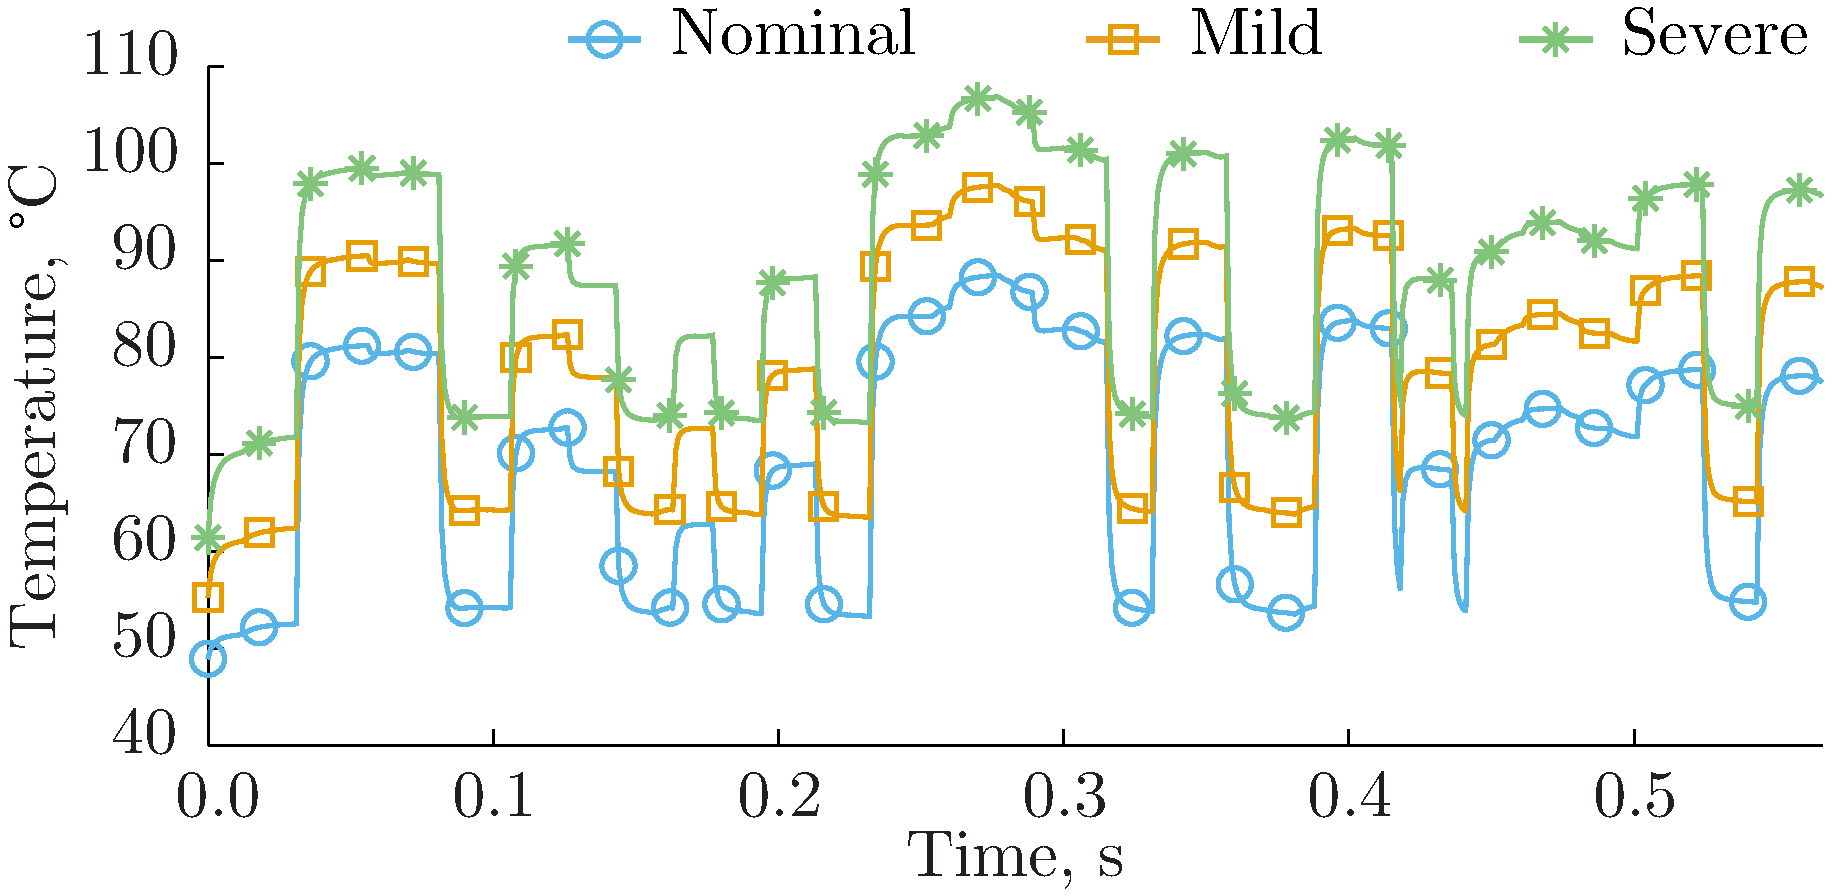
\includegraphics[width=1.0\linewidth]{include/assets/motivation-temperature.pdf}
  \vspace{-1.5em}
  \caption{Temperature fluctuation due to process variation.}
  \flabel{motivation-temperature}
\end{figure}

In order to illustrate the above concern, consider a quad-core architecture exposed to the uncertainty of the parameters that affect the leakage current.
Assume first that these parameters have nominal values.
We can then simulate the system under a certain workload and observe the corresponding temperature profile.\footnote{The experimental setup will be detailed in \sref{illustrative-example} and \sref{experimental-results}.}
The result, labeled as ``Nominal'', is depicted in \fref{motivation-temperature} where, for clarity, only one curve, corresponding to one processor, is presented (the bottom blue line). It can be seen that the temperature is always below $90^{\circ}$C.
Now let us assume a mild deviation of the parameters from the nominal values and run the simulation once again. The result is the ``Mild'' curve in \fref{motivation-temperature} (the middle orange line); the maximal temperature is approaching $100^{\circ}$C.
Finally, we repeat the experiment considering a severe deviation of the parameters and observe the curve labeled as ``Severe'' in \fref{motivation-temperature} (the top green line); the maximal temperature is almost $110^{\circ}$C.
Imagine that the designer, when tuning the solution constrained by a maximal temperature of $90^\circ$C, was guided exclusively by the nominal parameters.
In this case, even with mild deviations, the circuits might be burnt, and the amount of burnt circuits depends on the probability distribution of temperature.
Such uncertainties have to be addressed in order to pursue efficiency and fail-safeness.
Nevertheless, the majority of the literature related to power-temperature analysis of multiprocessor systems ignores this important aspect, \eg, \cite{rao2009, rai2011, thiele2011, ukhov2012}.

The remainder of the paper is organized as follows.
\sref{prior-work} provides an overview of the prior work.
In \sref{present-work}, we summarize the contribution of the present paper.
The objective of our study is formulated in \sref{problem-formulation}.
The proposed framework is presented in \sref{proposed-framework}.
A particular application of our approach is discussed in \sref{illustrative-example}, and the corresponding results are compared with MC simulations in \sref{experimental-results}.
\sref{conclusion} concludes the paper.
The work contains a set of supplementary materials with discussions on certain aspects of our framework.


  \section{Preliminaries}
  Throughout this article, we use the following notations. $\real$ and $\natural{n}$ are the set of real number and the set of integers greater or equal to $n$, respectively. Boldface letters denote vectors and matrices, e.g., $\m{M} = \mtx{m_{ij}} \in \real^{n \times m}$ is an $n \times m$ real matrix, and $\v{V} = \vec{v_i} \in \real^n$ is an $n$-dimensional real column vector. $\m{M}^T$ and $e^\m{M}$ are the transpose and matrix exponential of $\m{M}$, respectively. $\diag{m_i} \in \real^{n \times n}$ denotes an $n \times n$ diagonal matrix. $\mI_n$ is the $n \times n$ identity matrix, and $\mZero_{n \times m}$ is the $n \times m$ zero matrix; we shall omit these indexes when the actual dimensions of $\mI$ and $\mZero$ are clear from the context.

The tuple $(\outcomes, \sAlgebra, \pMeasure)$ denotes a complete probability space \cite{durrett2010} where $\outcomes$ is a set of outcomes, $\sAlgebra \subset 2^\outcomes$ is a $\sigma$-algebra on $\outcomes$, and $\pMeasure: \sAlgebra \to [0, 1]$ is a probability measure induced on the measurable space $(\outcomes, \sAlgebra)$. A $\sAlgebra$-measurable function $\rv{X}(\o): \outcomes \to \real$ is called a \definition{random variable} (r.v.). Denote $\exp_\rv{X} = \oExp{\rv{X}(\o)}$ the expectation of $\rv{X}(\o)$ and $\var_\rv{X} = \oVar{\rv{X}(\o)}$ its variance. A $\pMeasure$-measurable, vector-valued function $\mrv{X}(\o): \outcomes \to \real^n$ is called a random vector with $\vExp_\mrv{X} = \oExp{\mrv{X}(\o)}$ and $\mCov_\mrv{X} = \oCov{\mrv{X}(\o)}$ being its expectation vector and covariance matrix, respectively. A \definition{stochastic process} is a parametrized collection of r.v.'s $\{ \rv{X}(\t, \o) \}_{\t \in \sTime}$ where $\sTime$ is a parameter space, which is usually assumed to be the half line $[0, \infty)$ meaning time. $\{ \mrv{X}(\t, \o) \}_{\t \in \sTime}$ denotes a $n$-dimensional stochastic process.


  \section{System Model}
  \subsection{Architecture Model}
Consider a multiprocessor system that comprises $\cores$ processing elements of any kind and is equipped with a thermal package. Denote $\system$ the high-level \definition{description of the system} that includes the following information:
\begin{itemize}
  \item The floorplan of the die (the location and dimensions of the processing elements).
  \item The configuration of the thermal package (the dimensions of each of the layers).
  \item The thermal parameters of the materials that the die and package are made of (the thermal conductivity, specific heat, convection capacitance, and convection resistance).
\end{itemize}

Suppose the given system depends on a number of \definition{uncertain parameters}, i.e., r.v.'s that are possibly correlated. Let $(\outcomes, \sAlgebra, \pMeasure)$ be the corresponding probability space and $\vU(\o) = \vec{\param_i(\o)} \in \real^\params$, $\o \in \outcomes$, be a $\params$-dimensional vector of these parameters. Denote the expected value and covariance matrix of $\vU(\o)$ by $\vExp_\vU$ and $\mCov_\vU$, respectively.

In this work, we assume that the uncertainties $\vU(\o)$, $\o \in \outcomes$, are a result of the process variation and manifest themselves in the deviation of the actual power dissipation of the system from the nominal value. In this case, $\outcomes$ represents the outcomes of the manufacturing process that the given multiprocessor system is a product of. Without loss of generality, we focus at the leakage power as it is motivated in \sref{introduction}.

\subsection{Power Model}
The power dissipation of the system with $\cores$ processing elements at time $\t$ is modeled as
\[
  \vP(\t, \vTO(\t, \vU), \vU) = \vP_\dyn(\t) + \vP_\leak(\vTO(\t, \vU), \vU)
\]
where $\vP_\dyn, \vP_\leak \in \real^\cores$ are the dynamic and leakage power, respectively, and $\vTO \in \real^\cores$ is temperature. The leakage power is modeled as a function of temperature due to the well-known, strong interdependency between them.

\subsection{Thermal Model}
Given the system description $\system$, an equivalent thermal RC circuit with $\nodes$ \definition{thermal nodes} is constructed \cite{kreith2000}. The structure of the circuit depends on the intended level of details defining the accuracy of the final model.

The thermal behaviour of the circuit is modeled with the following system of differential-algebraic equations (DAEs) with the state-space dimension equal to $\nodes$:
\begin{align*}
  & \mC \frac{d\vTI(\t, \vU)}{d\t} + \mG \vTI(\t, \vU) = \mM \vP(\t, \vTO(\t, \vU), \vU) \\
  & \vTO(\t, \vU) = \mM^T \vTI(\t, \vU) + \vTO_\amb
\end{align*}
$\mC, \mG \in \real^{\nodes \times \nodes}$ are the matrices of the thermal capacitance and conductance, respectively. $\mC$ is a diagonal matrix with positive elements, and $\mG$ is a symmetric, positive-definite matrix. $\vTI \in \real^\nodes$ is the state vector of the system, which corresponds to the difference between the temperature of the thermal nodes and the ambient temperature. $\vP \in \real^\cores$ is the input vector of the power dissipation of the processing elements, and $\mM \in \real^{\nodes \times \cores}$ is its mapping matrix to the thermal nodes. $\vTO \in \real^\cores$ is the output vector of the system, which is the temperature of the processing elements. Finally, $\vTO_\amb \in \real^\cores$ is the vector of the ambient temperature, which, for clarity of presentation and without loss of generality, we model as a deterministic variable.

For convenience, we perform the following transformation of the original system. Let $\vX = \mC^{1/2} \vTI$, $\mA = \mC^{1/2} \mG \mC^{1/2}$, and $\mB = \mC^{1/2} \mM$, then
\begin{align}
  & \frac{d\vX(\t, \vU)}{d\t} = \mA \vX(\t, \vU) + \mB \vP(\t, \vTO(\t, \vU), \vU) \elabel{fourier} \\
  & \vTO(\t, \vU) = \mB^T \vX(\t, \vU) + \vTO_\amb \nonumber
\end{align}
where $\vX$ is the new state vector. It can be seen that the coefficient matrix $\mA$ preserves the properties of $\mG$, i.e., it is symmetric and positive-definite.

\subsection{System Profiles}
A \definition{power profile} of the system over a time interval $\period$ is defined as a tuple $\pP$. $\pTime = \{ 0 = \t_0 < \dots < \t_{\steps} = \period \}$ is a partition of $\period$ into $\steps$ subintervals $\dt_i = \t_{i+1} - \t_i$. $\mP \in \real^{\cores \times \steps}$ is a matrix of the corresponding power dissipation where the $i$th column vector, $\vP_i \in \real^\cores$, represents the power consumption of the processing elements at the \emph{beginning} of the $i$th time interval, $\dt_i$.

A \definition{temperature profile} of the system with respect to $\pP$ is defined as a tuple $\pT$. $\pTime$ remains the same as for the power profile, and $\mTO \in \real^{\cores \times \steps}$ is a matrix of the corresponding temperature where the $i$th column vector, $\vTO_i \in \real^\cores$, represents the temperature of the processing elements at the \emph{end} of the $i$th time interval, $\dt_i$.


  \bibliographystyle{unsrt}
  \bibliography{include/references}
\end{document}
